\documentclass{beamer}
\PassOptionsToClass{handout}{beamer}


\usetheme{Madrid}

\usepackage{graphicx}
\usepackage{hyperref}
\usepackage{subcaption}
\usepackage{float}
\usepackage{csquotes}
\usepackage{pifont}
\setbeamertemplate{navigation symbols}{}
\usepackage[ngerman]{babel}
\usepackage[style=verbose,backend=bibtex]{biblatex}
\usepackage{algorithm}
\usepackage{algpseudocode}
\setbeamertemplate{footline}
{
  \leavevmode%
  \hbox{%
  \begin{beamercolorbox}[wd=.333333\paperwidth,ht=2.25ex,dp=1ex,center]{author in head/foot}%
    \usebeamerfont{author in head/foot}Ian Schmetkamp%\insertshortauthor
  \end{beamercolorbox}%
  \begin{beamercolorbox}[wd=.333333\paperwidth,ht=2.25ex,dp=1ex,center]{title in head/foot}%
    \usebeamerfont{title in head/foot}Autonomous Object Inspection
  \end{beamercolorbox}%
  \begin{beamercolorbox}[wd=.333333\paperwidth,ht=2.25ex,dp=1ex,right]{date in head/foot}%
    \usebeamerfont{date in head/foot}\insertshortdate{}\hspace*{2em}
    \insertframenumber{} / \inserttotalframenumber\hspace*{2ex}
  \end{beamercolorbox}}%
  \vskip0pt%
}
\title{Autonomous Object Inspection with Mobile Robots for 3D Reconstruction and Image Data Acquisition}
\author{Ian Schmetkamp \inst{1} \\ \textbf{Advisor:} Philip Keller \inst{2} \\ \textbf{Supervisor:} Prof. Dr.-Ing. Rüdiger Dillmann \inst{2}}
\subtitle{Bachelor Thesis}
\institute{Karlsruhe Institute of Technology \and FZI Research Center for Information Technology}
\date{\today}

\bibliography{references.bib}
\begin{document}
\frame{\titlepage}
\frame{\frametitle{Inhalt}\tableofcontents}

\section{Allgemeines}
\begin{frame}{Aufgabe}
	\begin{minipage}{0.55 \textwidth}
		\begin{block}{Ziel}
			\begin{itemize}
				\item autonom Bilder von Object aufnehmen
				\item Bilder aus verschiedenen Perspektiven
				\item \textbf{Roboter (Spot, Turtlebot, etc.) muss nächste, vorteilhafte Perspektive berechnen}
			\end{itemize}
		\end{block}
	\end{minipage}
	\hfill
	\begin{minipage}{0.4 \textwidth}
		\centering
		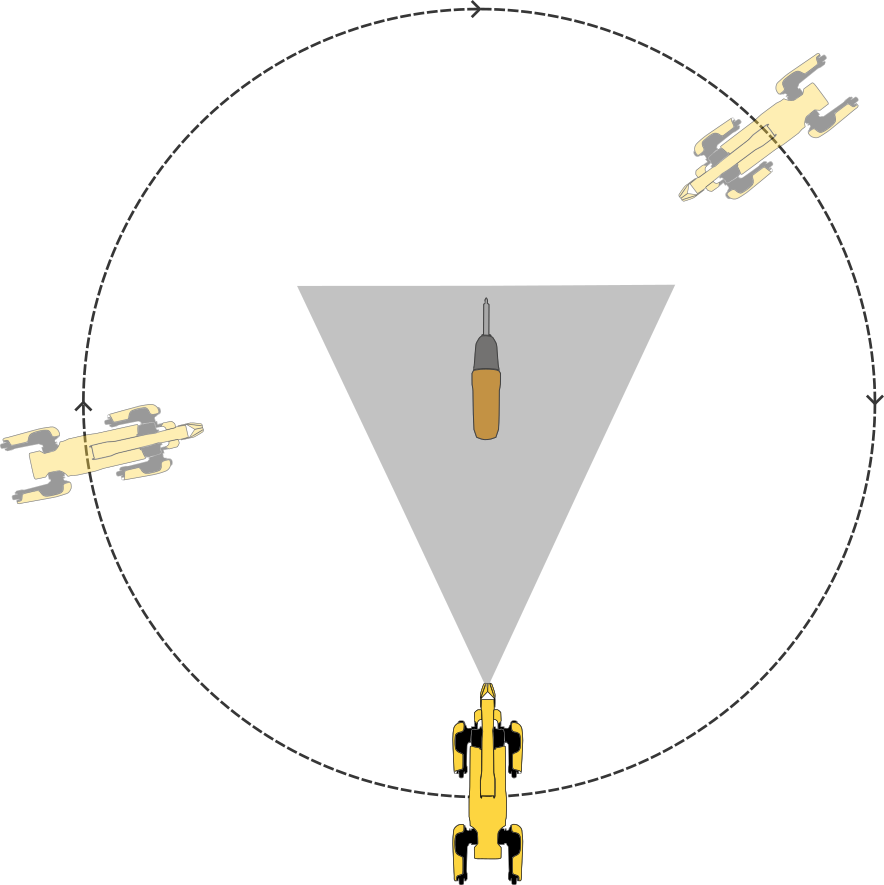
\includegraphics[width=1\textwidth]{Graphics/graphic_top_down.png}
	\end{minipage}
\end{frame}

\begin{frame}{Ansatz}
	\begin{block}{Ansatz}
		\begin{itemize}
			\item Mögliche Positionen evaluieren
			\item Abschätzen wie viel Informationen in möglicher Position gesehen wird (Stichwort: Next-Best-View)
			\item Andere Faktoren für Positionen evaluieren (Distanz, Überlappung, Sichtbarkeit des Bekannten etc.)
			\item Zur besten Position gehen
		\end{itemize}
	\end{block}
	\begin{center}
		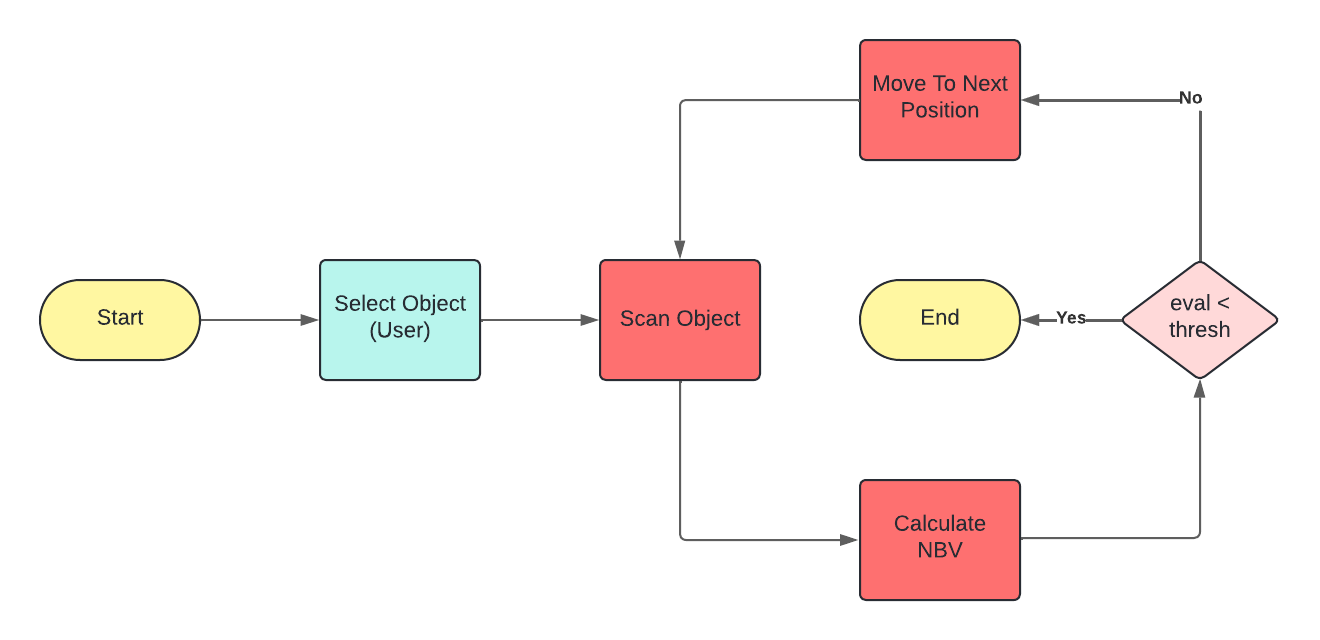
\includegraphics[width=0.7\textwidth]{Graphics/flow_chart_v2.png}
	\end{center}
\end{frame}

\section{Algorithmen}
\begin{frame}{Algorithmen}
	\begin{algorithm}[H]
		\caption{NBV}
		\begin{algorithmic}[1]
			\Require pixel: Tuple$<$int$ >$, thresh
			\State ray = convertPixelToRay(pixel)
			\State scan()
			\State origin = raytrace(camera.position, ray)
			\While{eval $>$ thresh}
			\State scan()
			\State surfaceVoxel, frontierVoxel =  breadthFirstSearch(origin)
			\State frontiers = groupFrontiers(frontierVoxel)
			\State candidates = generateCandidates(frontiers)
			\State eval, c = max(evaluateCandidates(candidates, surfaceVoxel))
			\State moveTo(c)
			\EndWhile
		\end{algorithmic}
	\end{algorithm}
\end{frame}
\begin{frame}{Definitionen}
	\begin{exampleblock}{Visible unknown Voxel}
		\begin{itemize}
			\item unbekannte Voxel, die von einem anderen Punkt als erste gesehen werden
			\item unbekannte Voxel benachbart zu einem freien Voxel
			\item eingeführt von Vasquez et al.\footcite{vasquez-gomez_vpl_2020}
		\end{itemize}
	\end{exampleblock}
	\begin{exampleblock}{Frontier Voxel}
		\begin{itemize}
			\item visible unknown Voxel, die benachbart zu besetzen Voxel sind
			\item benachbarte Frontier Voxel bilden eine Frontier

		\end{itemize}
	\end{exampleblock}
\end{frame}

\begin{frame}{}
	\centering
	\begin{figure}
		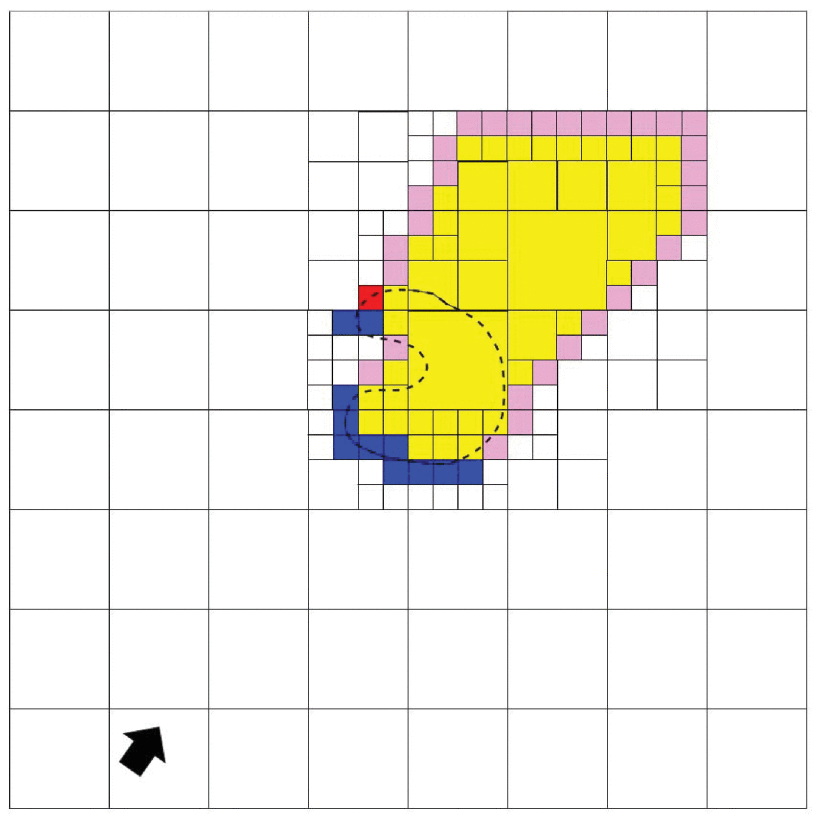
\includegraphics[width=0.5\textwidth]{Graphics/vasquez.png}
		\caption{occupied voxel blue, unknown voxel yellow, \textbf{visible unknown} voxel pink, \textbf{frontier} voxel red, }\footcite{vasquez-gomez_vpl_2020}
	\end{figure}
\end{frame}

\begin{frame}{Algorithmen}
	\begin{exampleblock}{Frontier Voxel}
		\begin{itemize}
			\item unbekannte Voxel, die benachbart zu freien \textbf{und} besetzen Voxel sind
			\item benachbarte Frontier Voxel bilden eine Frontier
		\end{itemize}
	\end{exampleblock}

	\begin{block}{1. Breitensuche}
		\begin{itemize}
			\item Finde alle besetzen Voxel, die über besetze Voxel mit Origin verbunden sind
			\item Findet die bisher bekannte Oberfläche
			\item Filtert den Boden heraus
			\item Markiert alle gefundenen unbekannte Voxel die freien Nachbarn haben
		\end{itemize}
	\end{block}
\end{frame}

\begin{frame}{Algorithmen}
	\begin{exampleblock}{Frontier Voxel}
		\begin{itemize}
			\item unbekannte Voxel, die benachbart zu freien \textbf{und} besetzen Voxel sind
			\item benachbarte Frontier Voxel bilden eine Frontier
		\end{itemize}
	\end{exampleblock}
	\begin{block}{2. Breitensuche: Frontier Voxel gruppieren}
		\begin{itemize}
			\item 2 verschachtelte Breitensuchen
			\item gruppiert alle benachbarten Frontier Voxel zu einer Frontier
			\item Berechnet Zentrum der Frontier
		\end{itemize}
	\end{block}
\end{frame}

\begin{frame}{Algorithmen}
	\begin{block}{Kandidaten Positionen generieren}

	\end{block}

\end{frame}

\begin{frame}{Algorithmen}
	\begin{algorithm}[H]
		\caption{Evaluate Candidates Part 1}
		\begin{algorithmic}[2]
			\Require candidates, surfaceVoxel
			\For{c $\in$ candidates}
			\State num\_surface, num\_seen\_surface, num\_seen\_unknown = 0
			\For{s $\in$ surfaceVoxel}
			\If{isPartOfViewFrustum(s, c)}
			\State num\_surface++
			\EndIf
			\EndFor
			\EndFor

		\end{algorithmic}
	\end{algorithm}

\end{frame}

\begin{frame}{Algorithmen}
	\begin{algorithm}[H]
		\caption{Evaluate Candidates Part 2}
		\begin{algorithmic}[2]
			\Require candidates, surfaceVoxel
			\For{c $\in$ candidates}
			\For{pixel $\in$ Sensor}
			\State ray = rotateToPose(convertPixelToRay(pixel), c)
			\State point = {\color{blue}raytraceInRange(c, ray)}
			\If {point $\in$ surfaceVoxel}
			\State num\_seen\_surface++
			\EndIf
			\If {point is unknown}
			\State num\_seen\_unknown++
			\EndIf
			\EndFor
			\EndFor

		\end{algorithmic}
	\end{algorithm}

\end{frame}

\begin{frame}{Evaluation}
	\begin{block}{}
		Für ein Kandidaten $v$:
		\[f(v) = \cfrac{1}{1 + \text{d(v)}} \cdot \cfrac{\text{num\_seen\_unknown(v)}}{1 + \text{max\_seen\_unknown(v)}} \cdot (\cfrac{\text{num\_surface(v)}}{\text{num\_surface(v)}})^2 \cdot r(v) \cdot p(v)\]
		Mit \[p(v) = \begin{cases}
				1 & \quad \text{Wenn } v \text{ erreichbar ist} \\
				0 & \quad \text{sonst}
			\end{cases}\]
		und \[r(v) = \begin{cases}
				1 & \quad \text{Wenn  num\_surface\_seen} > \text{surfaceVoxel.size()} \cdot 0.1 \\
				0 & \quad \text{sonst}
			\end{cases}
		\]
	\end{block}
\end{frame}
\section{Probleme}
\begin{frame}{Problem: Unknown Barrier}

\end{frame}
\end{document}
